%==================================================================================================
\subsection{Exemplos Numéricos} \label{ExemplosMT}
%==================================================================================================

Na presente seção serão apresentadas algumas simulações realizadas utilizando os modelos VMS e LES, com a finalidade de validar os modelos implementados.

%==================================================================================================
\subsubsection{Cavidade bidimensional}
%==================================================================================================

A primeira simulação considerada trata-se de uma cavidade quadrada ($\Omega=[-1,1]^2$) com paredes aderentes, onde o fluido encontra-se confinado e sujeito a uma velocidade prescrita $\BB{u}_\infty$ ocasionada devido ao deslizamento de uma parede na face superior da cavidade. Nesse sentido serão observados os efeitos provocados no fluido devido à diferentes números de Reynolds, o qual é calculado por meio da equação \ref{eq:Reynolds}:

\begin{equation}
    \Rey=\frac{\rho L\norm{\BB{u}_\infty}}{\mu}\text{,}
    \label{eq:Reynolds}
\end{equation}

\noindent em que $L$ é o comprimento característico, que no caso analisado é igual ao lado da cavidade. Dessa forma considera-se uma velocidade constante para todas as análises de $\BB{u}_\infty=\{1,0\}^T$, sendo os diferentes números de Reynolds obtidos pela variação da viscosidade do fluido. A Figura \ref{fig:cavity} apresenta esquematicamente o problema simulado.

\begin{figure}[h!]
    \centering
    \caption{Desenho esquemático do problema de cavidade.}
    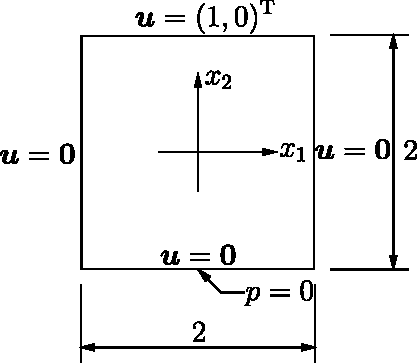
\includegraphics[width=.35\linewidth]{Figuras/Cavity/cavidade.pdf}
    \\Fonte: Autoria Própria (\the\year).
    \label{fig:cavity}
\end{figure}

Pelo fato do problema possuir apenas fronteiras do tipo Dirichlet, o condicionamento da solução do campo de pressões é garantido pela aplicação de uma condição de pressão nula no vértice superior direito da cavidade, conforme visto na figura acima.  Também se observa que existe uma descontinuidade nas condições de contorno no encontro entre as paredes da cavidade e seu topo, podendo ser consideradas velocidades nulas ou igual à velocidade do topo. No problema em questão considerou-se que a velocidade nesse ponto é igual à $\BB{u}_\infty$.

A malha de elementos finitos foi feita pela subdivisão do domínio em 20000 elementos dispostos de maneira estruturada com orientação à esquerda, conforme observado na Figura \ref{fig:cavity_disc}. O número de graus de liberdade para a simulação VMS de aproximação linear, quadrática e LES são 30603, 121203 e 91003, respectivamente. Os parâmetros utilizados foram $\rho=1$ para todas as análises, $\mu=0,02$, $\mu=5\times10^{-3}$, $\mu=2\times10^{-3}$, $\mu=4\times10^{-4}$, $\mu=2,6667\times10^{-4}$ e $\mu=2\times10^{-4}$, resultando em $\Rey=100$, $\Rey=400$, $\Rey=1000$, $\Rey=5000$, $\Rey=7500$ e $\Rey=10000$, respectivamente. Os modelos utilizados foram o VMS com aproximação linear e quadrática e o LES com elementos de Taylor-Hood P2P1 e $C_S=0,10$. O passo de tempo em todos os casos foi de $\Delta t=0,1$ e a simulação foi mantida até que a estacionariedade dos parâmetros do fluxo fosse alcançada.

\begin{figure}[h!]
    \centering
    \caption{Malha considerada para o problema de cavidade.}
    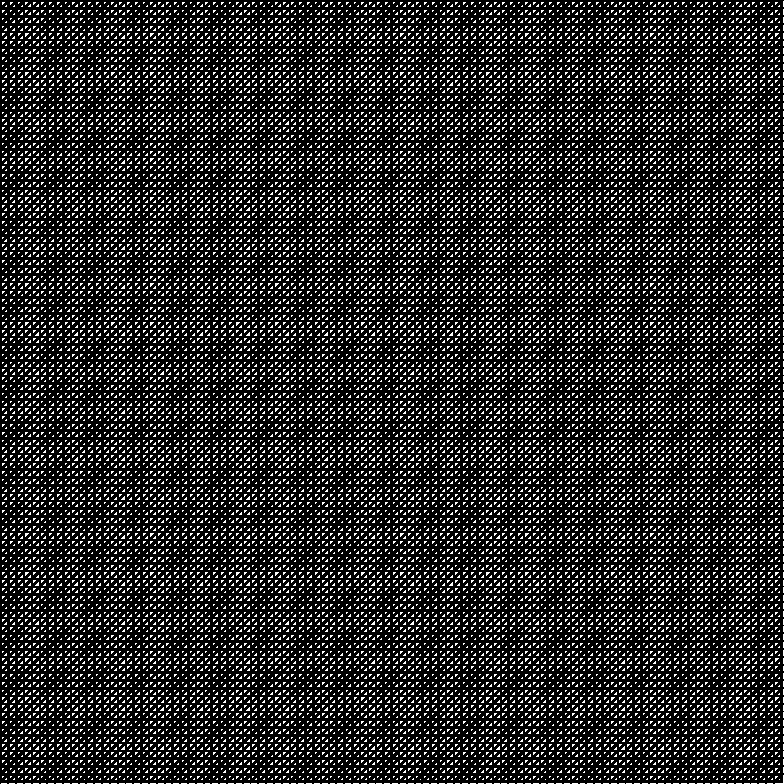
\includegraphics[width=.6\linewidth]{Figuras/Cavity/mesh.pdf}
    \\Fonte: Autoria Própria (\the\year).
    \label{fig:cavity_disc}
\end{figure}

Como o problema apresenta características de um escoamento quase-estático, a parcela dos termos inerciais foram desprezados em ambos os modelos de turbulência. Além disso, os resultados adquiridos para um determinado número de Reynolds foram aplicados como valores iniciais para a determinação dos resultados para a próxima análise.

Os resultados obtidos foram comparados com aqueles apresentados por \citeonline{ghia1982high}. A Figura \ref{fig:cavity-results} apresenta os valores do campo de velocidades sobre as linhas médias da cavidade ($x_1=0$ e $x_2=0$).

\begin{figure}[h!]
    \centering
    \caption{Valores do campo de velocidades sobre as linhas médias da cavidade.}
    \begin{subfigure}{0.4\textwidth}
        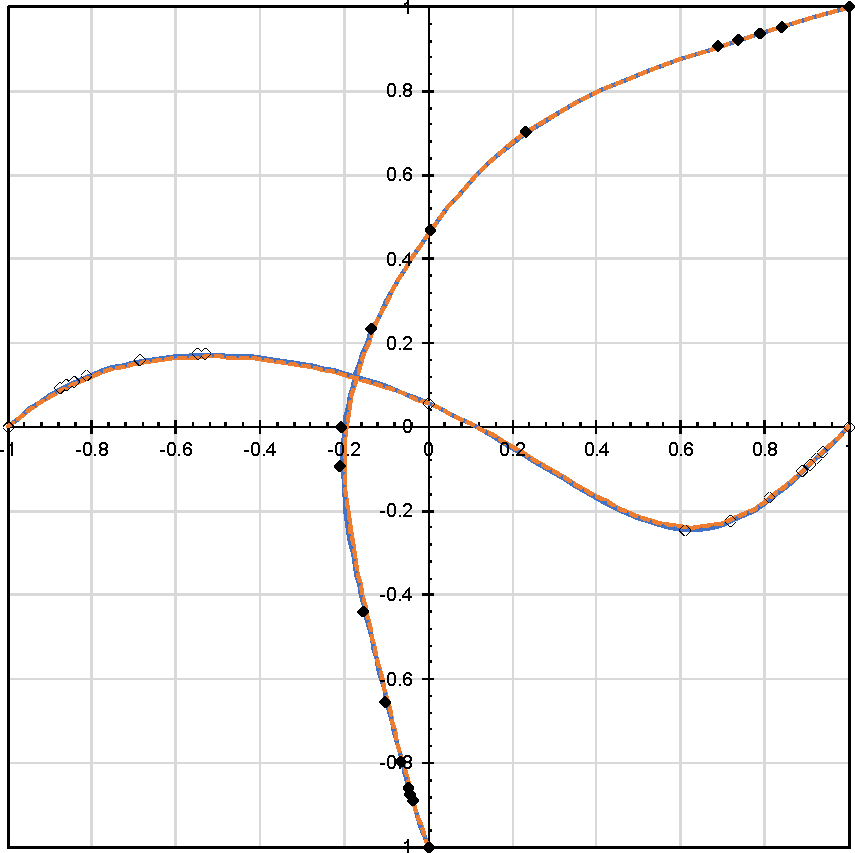
\includegraphics[width=\linewidth]{Figuras/Cavity/Re100.pdf}
        \caption{$\Rey=100$}
    \end{subfigure}
    \begin{subfigure}{0.4\textwidth}
        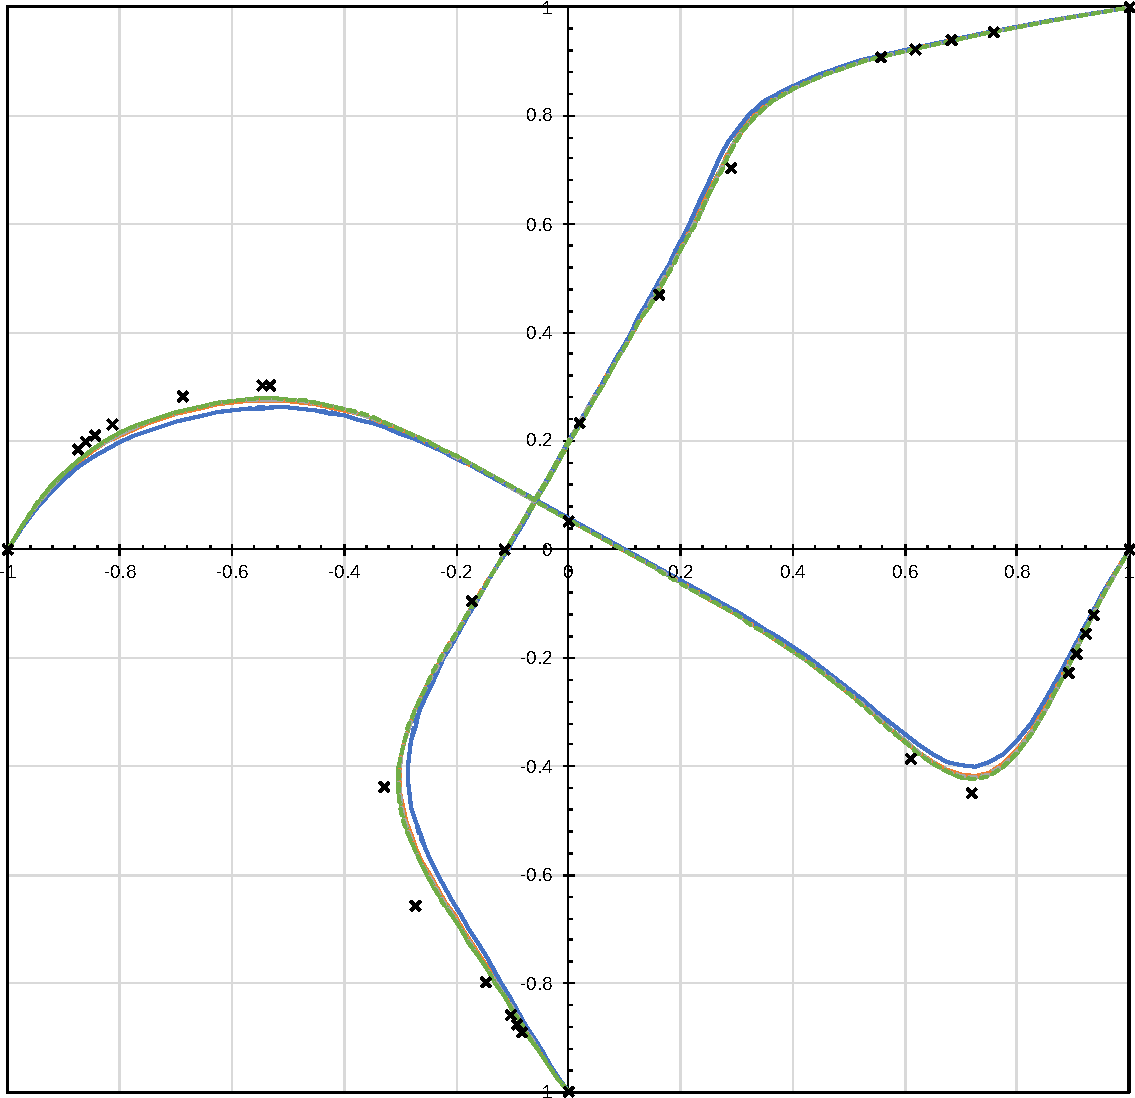
\includegraphics[width=\linewidth]{Figuras/Cavity/Re400.pdf}
        \caption{$\Rey=400$}
    \end{subfigure}
    \begin{subfigure}{0.4\textwidth}
        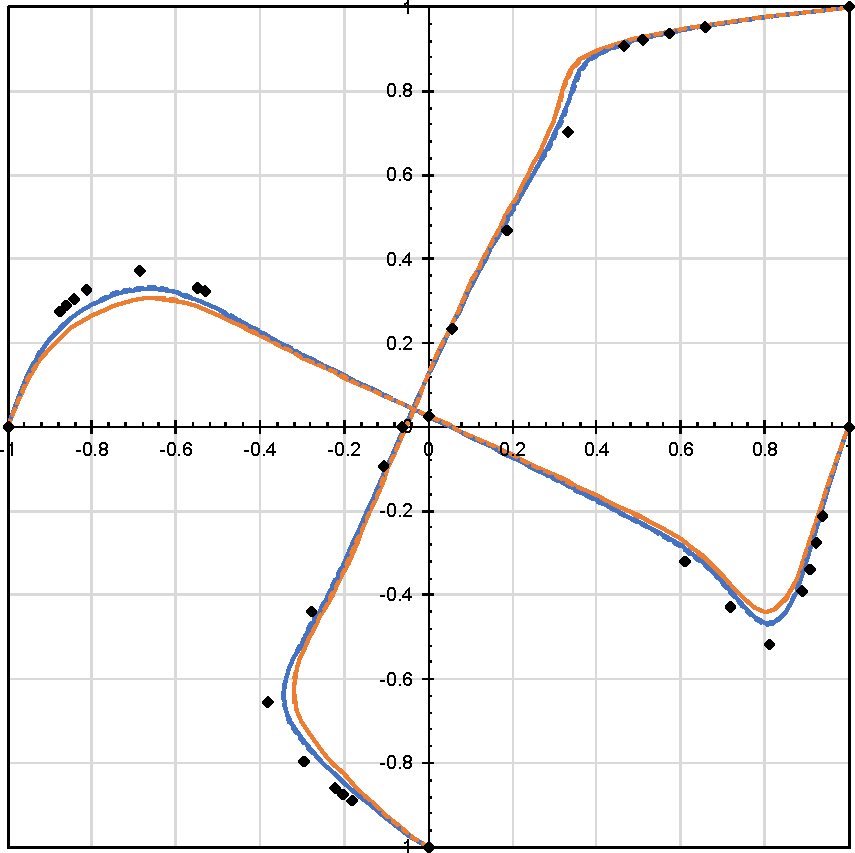
\includegraphics[width=\linewidth]{Figuras/Cavity/Re1000.pdf}
        \caption{$\Rey=1000$}
    \end{subfigure}
    \begin{subfigure}{0.4\textwidth}
        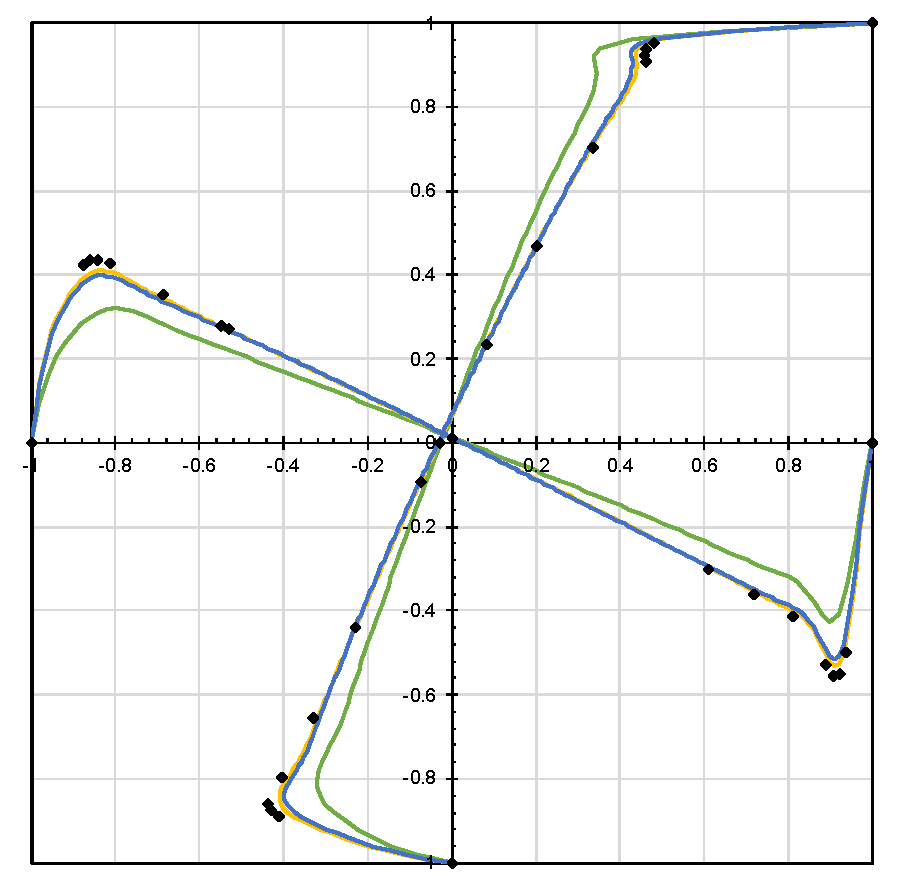
\includegraphics[width=\linewidth]{Figuras/Cavity/Re5000.pdf}
        \caption{$\Rey=5000$}
    \end{subfigure}
    \begin{subfigure}{0.4\textwidth}
        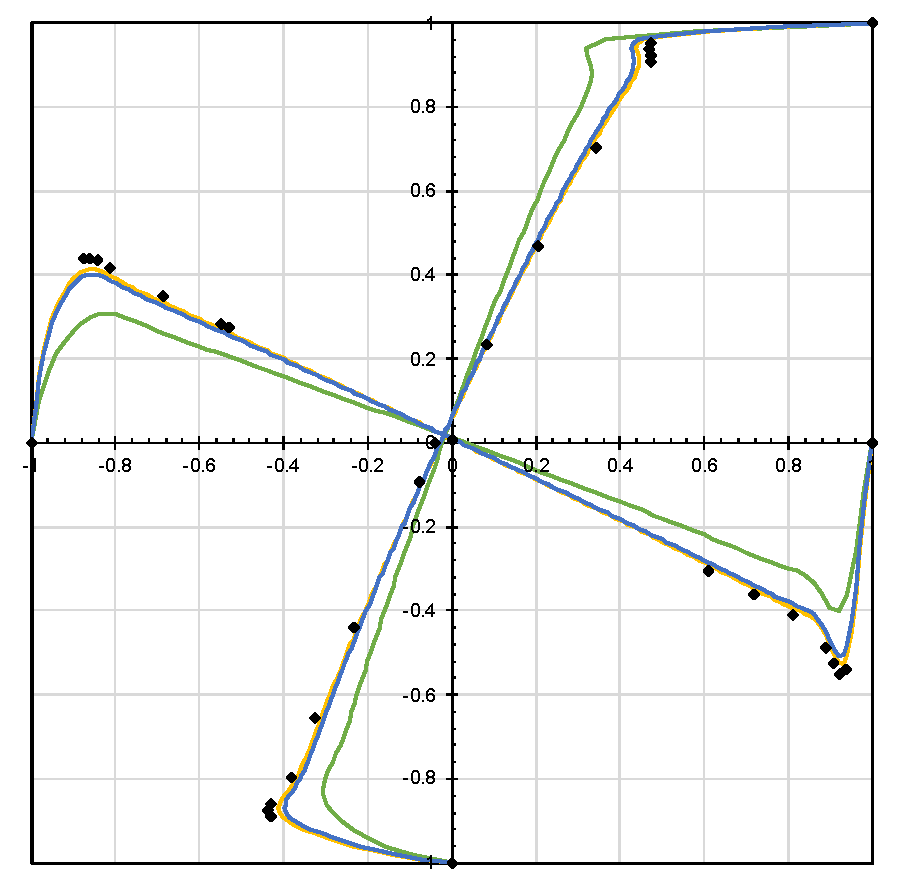
\includegraphics[width=\linewidth]{Figuras/Cavity/Re7500.pdf}
        \caption{$\Rey=7500$}
    \end{subfigure}
    \begin{subfigure}{0.4\textwidth}
        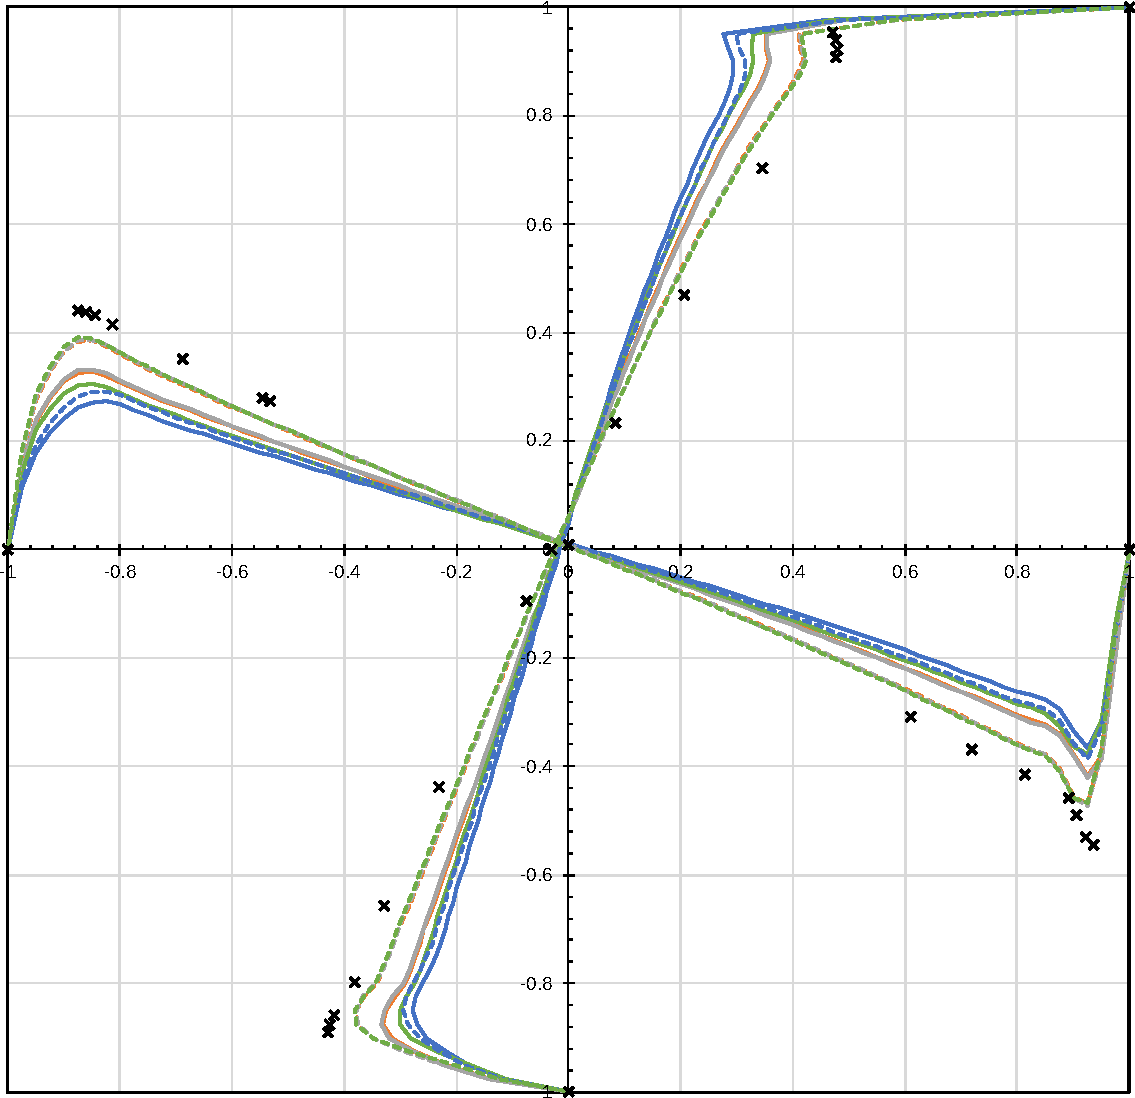
\includegraphics[width=\linewidth]{Figuras/Cavity/Re10000.pdf}
        \caption{$\Rey=10000$}
    \end{subfigure}
    \begin{subfigure}{\textwidth}
        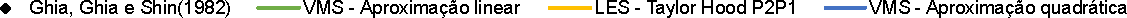
\includegraphics[width=\linewidth]{Figuras/Cavity/Legenda.pdf}
    \end{subfigure}
    \\Fonte: Autoria Própria (\the\year).
    \label{fig:cavity-results}
\end{figure}

A Figura \ref{fig:cavity-results2} apresenta o campo de velocidades na cavidade após o escoamento atingir seu estado estacionário.

\begin{figure}[h!]
    \centering
    \caption{Campo de velocidades em regime estacionário na cavidade.}
    \begin{subfigure}{0.32\textwidth}
        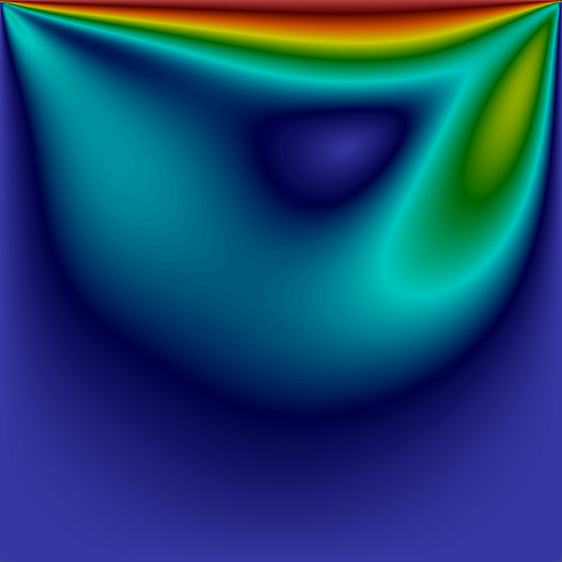
\includegraphics[width=\linewidth]{Figuras/Cavity/Re100.png}
        \caption{$\Rey=100$}
    \end{subfigure}
    \begin{subfigure}{0.32\textwidth}
        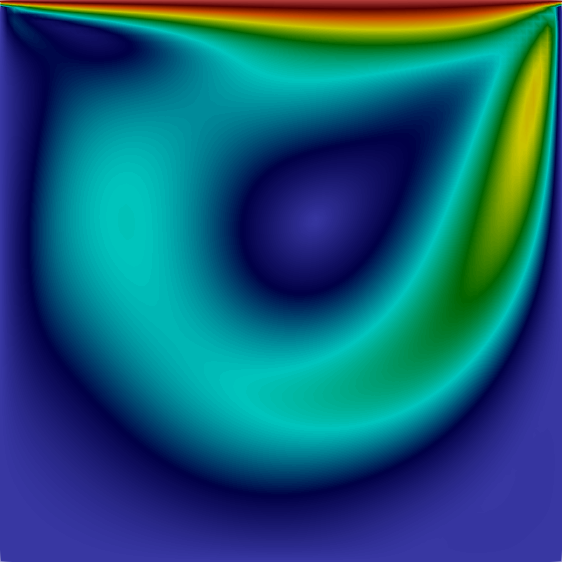
\includegraphics[width=\linewidth]{Figuras/Cavity/Re400.png}
        \caption{$\Rey=400$}
    \end{subfigure}
    \begin{subfigure}{0.32\textwidth}
        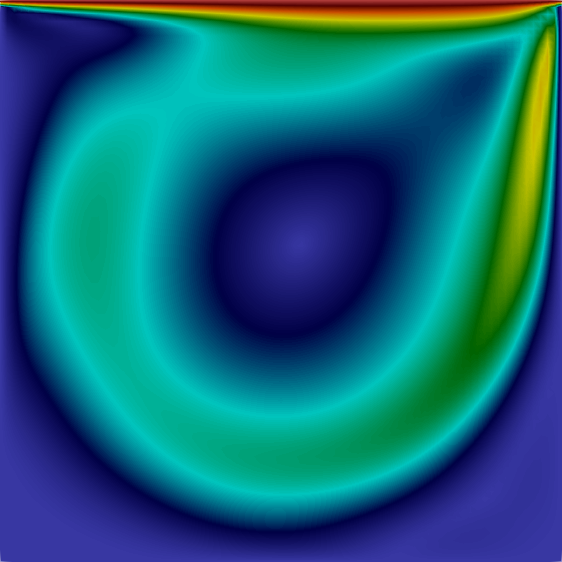
\includegraphics[width=\linewidth]{Figuras/Cavity/Re1000.png}
        \caption{$\Rey=1000$}
    \end{subfigure}
    \begin{subfigure}{0.32\textwidth}
        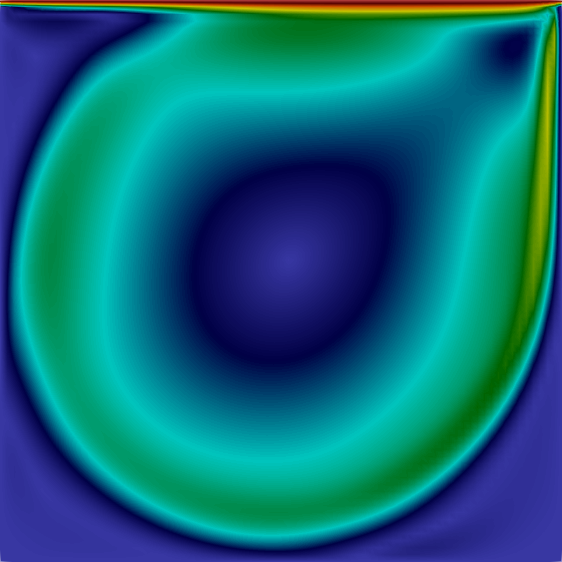
\includegraphics[width=\linewidth]{Figuras/Cavity/Re5000.png}
        \caption{$\Rey=5000$}
    \end{subfigure}
    \begin{subfigure}{0.32\textwidth}
        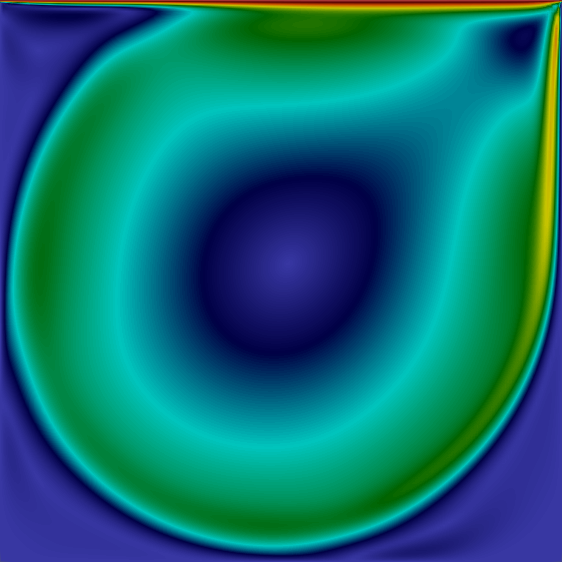
\includegraphics[width=\linewidth]{Figuras/Cavity/Re7500.png}
        \caption{$\Rey=7500$}
    \end{subfigure}
    \begin{subfigure}{0.32\textwidth}
        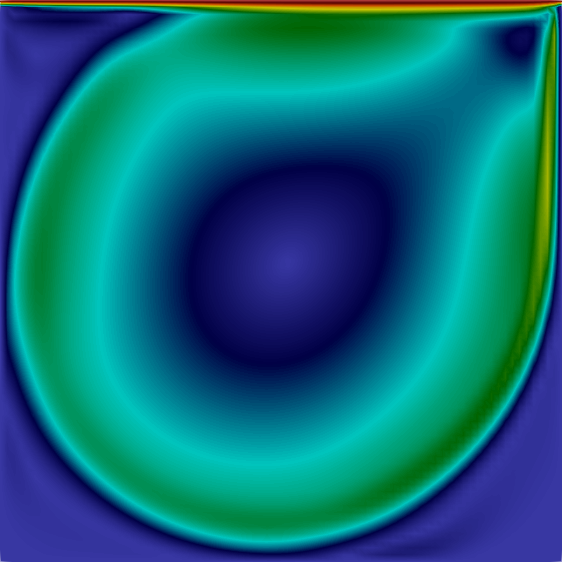
\includegraphics[width=\linewidth]{Figuras/Cavity/Re10000.png}
        \caption{$\Rey=10000$}
    \end{subfigure}
    \begin{subfigure}{0.4\textwidth}
        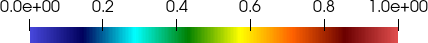
\includegraphics[width=\linewidth]{Figuras/Cavity/Legenda.png}
    \end{subfigure}
    \\Fonte: Autoria Própria (\the\year).
    \label{fig:cavity-results2}
\end{figure}

Para todas as simulações conduzidas, percebeu-se que houve uma excelente concordância dos resultados para números de Reynolds baixos, no entanto a simulação VMS de aproximação linear passou a apresentar resultados cada vez mais discrepantes à medida que o número de Reynolds aumentou, enquanto o VMS de aproximação quadrática e o LES apresentaram resultados mais próximos aos de \citeonline{ghia1982high}, sendo que o LES apresentou resultados ligeiramente melhores em relação ao VMS quadrático. Para número de Reynolds muito altos observou-se um leve desvio nos resultados próximos à parede superior da cavidade, o que poderia ser melhorado caso uma discretização mais fina da malha fosse empregada nessa região.

\textcolor{red}{Fazer análise da convergência dos métodos e o tempo de processamento.}

%==================================================================================================
\subsubsection{\textit{Taylor-Green Vortex} tridimensional}
%==================================================================================================

Para verificação dos modelos implementados em simulações tridimensionais é possível simular o problema de \textit{Taylor-Green Vortex} (TGV), o qual possui solução analítica, dada por \cite{shapiro1993use}:

\begin{subequations}
    \begin{equation}
        \begin{split}
            &\BB{u}_a(\BB{x},t)=\\
            &-\frac{Ae^{-\nu\lambda^2t}}{k^2+l^2}\begin{bmatrix}
                \lambda l\cos{(kx_1)}\sin{(lx_2)}\sin{(mx_3)}+mk\sin{(kx_1)}\cos{(lx_2)}\cos{(mx_3)} \\
                \lambda k\sin{(kx_1)}\cos{(lx_2)}\sin{(mx_3)}-ml\cos{(kx_1)}\sin{(lx_2)}\cos{(mx_3)} \\
                -(k^2+l^2)\cos{(kx_1)}\cos{(lx_2)}\sin{(mx_3)}
            \end{bmatrix}\text{,}
        \end{split}
    \end{equation}
    \begin{equation}
        p_a=p_s-\rho\frac{u_1^2+u_2+u_3^2}{2}\text{.}
    \end{equation}
\end{subequations}

\noindent em que $k$, $l$ e $m$ são constantes arbitrárias, $\lambda^2=k^2+l^2+m^2$, $A$ é a amplitude da componente $u_3$ e $p_s$ é a pressão do ponto de estagnação.

Para o problema numérico foi considerado um cubo ($\Omega=[-1,1]^3$) simulado nos modelos VMS de aproximação linear e quadrática e o LES utilizando elementos Taylor-Hood P2P1. A malha utilizada na discretização conta com 5802 elementos finitos (conforme ilustrado na Figura \ref{fig:TGV-mesh}), sendo 5580 graus de liberdade para VMS linear, 37600 pra VMS quadrático e 29595 para LES.

\begin{figure}[h!]
    \centering
    \caption{Malha utilizada para a simulação de TGV.}
    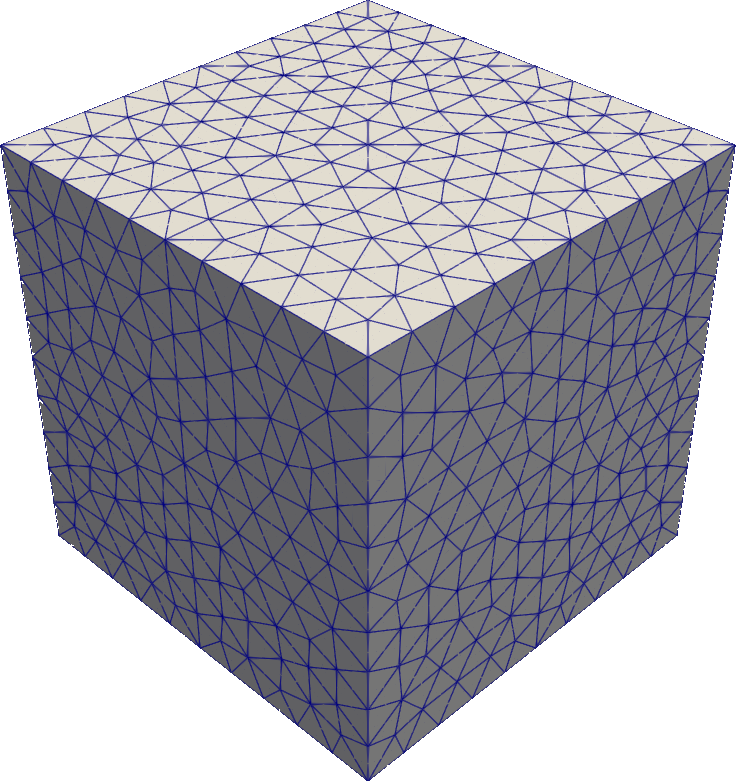
\includegraphics[width=0.4\linewidth]{Figuras/taylor-green/mesh.png}
    \\Fonte: Autoria Própria (\the\year).
    \label{fig:TGV-mesh}
\end{figure}

Como condição inicial impôs-se acelerações, velocidade e pressões iguais à solução analítica com $t=0$ e como condições de contorno aplicou-se velocidades iguais à analítica em toda a fronteira e $p=0$ no centro do domínio. Os valores dos parâmetros foram $k=l=m=\pi$ e $A=\nu=\rho=1$, sendo o período analisado de $t\in[0,0.2]$ com um passo de tempo de $\Delta t=0.001$.

Sendo assim, a Figura \ref{fig:TGV-results} apresenta os valores do campo de velocidades nas linhas $u_2=u_3=0$ ($l1$), $u_1=u_3=0$ ($l2$) e $u_1=u_2=0$ ($l3$) para os instantes $t=0$, $t=0.05$ e $t=0.2$ para todos os modelos considerados.

\begin{figure}[h!]
    \centering
    \caption{Resultados obtidos para a simulação de TGV em:}
    \begin{subfigure}{0.42\textwidth}
        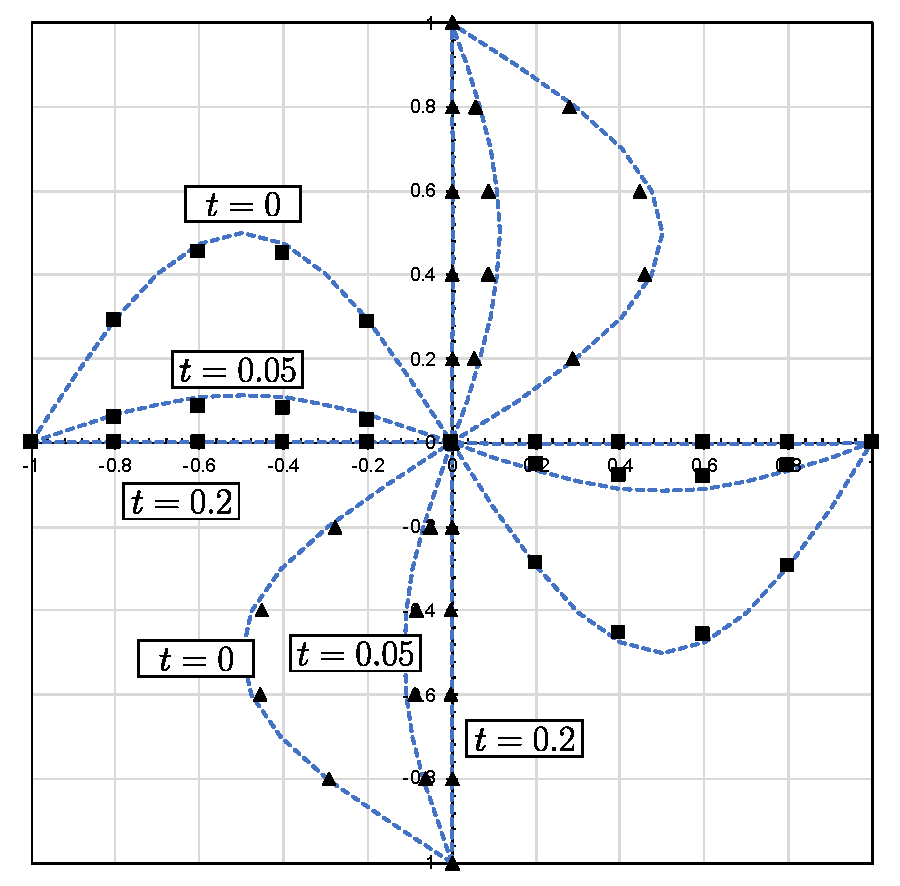
\includegraphics[width=\linewidth]{Figuras/taylor-green/VMS-Lin.pdf}
        \caption{$l1$ e $l2$ para VMS linear.}
    \end{subfigure}
    \begin{subfigure}{0.42\textwidth}
        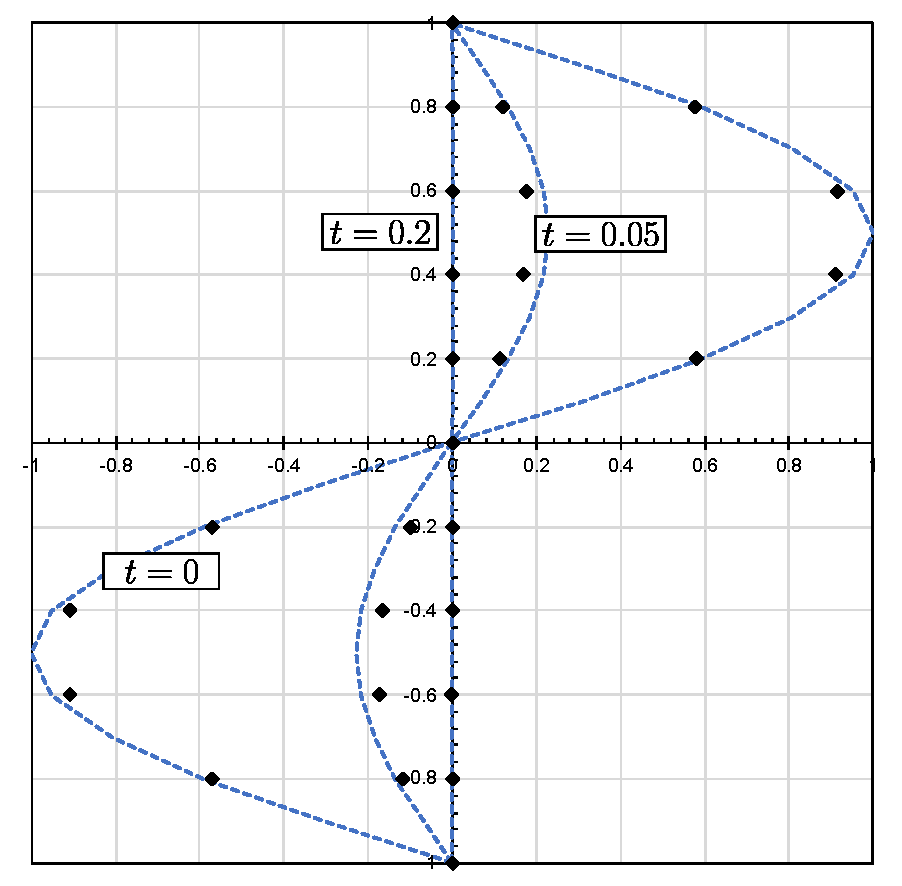
\includegraphics[width=\linewidth]{Figuras/taylor-green/VMS-Lin-uz.pdf}
        \caption{$l3$ para VMS linear.}
    \end{subfigure}
    \begin{subfigure}{0.42\textwidth}
        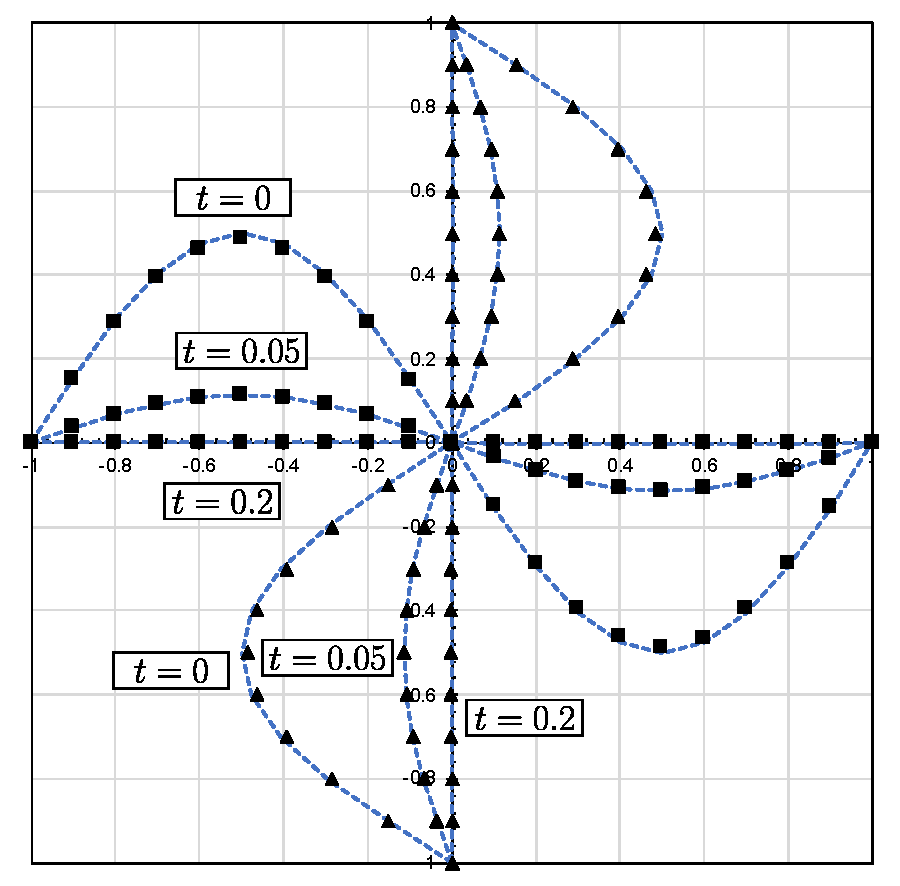
\includegraphics[width=\linewidth]{Figuras/taylor-green/VMS-Qua.pdf}
        \caption{$l1$ e $l2$ para VMS quadrático.}
    \end{subfigure}
    \begin{subfigure}{0.42\textwidth}
        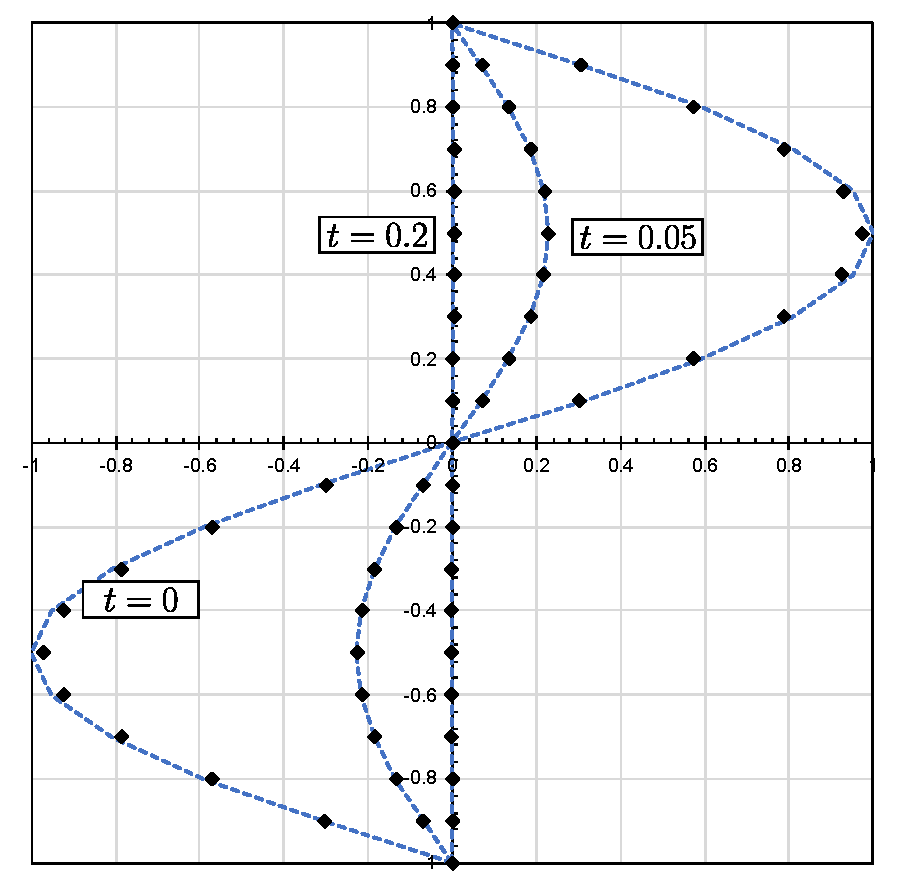
\includegraphics[width=\linewidth]{Figuras/taylor-green/VMS-Qua-uz.pdf}
        \caption{$l3$ para VMS quadrático.}
    \end{subfigure}
    \begin{subfigure}{0.42\textwidth}
        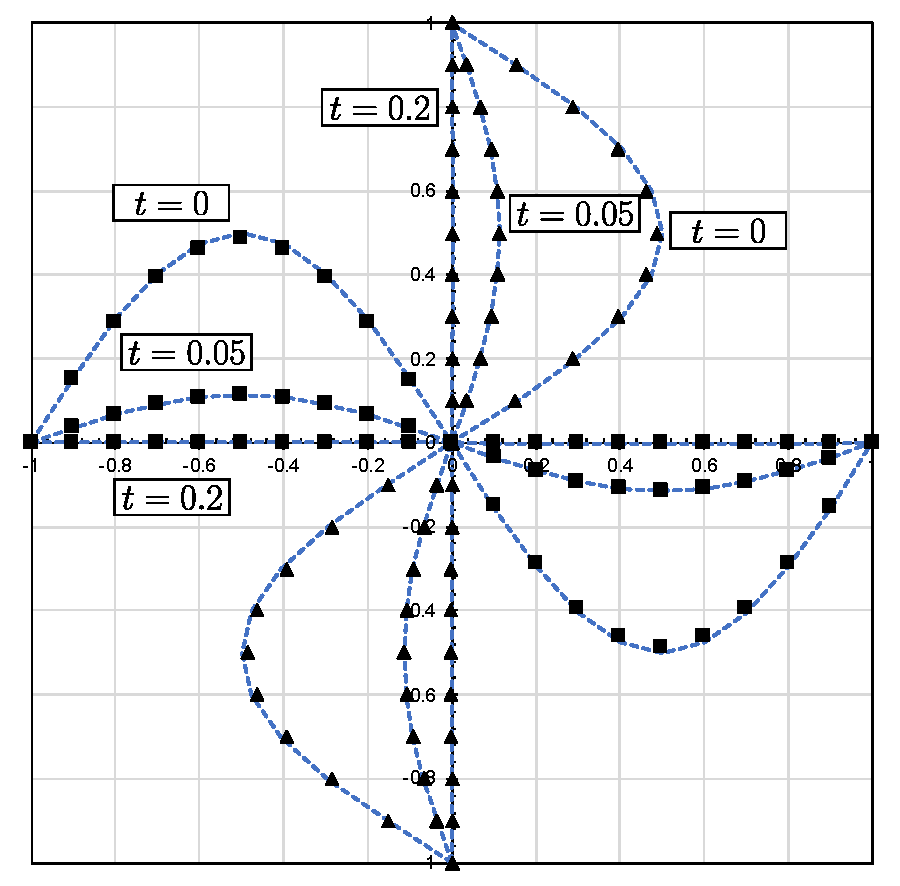
\includegraphics[width=\linewidth]{Figuras/taylor-green/LES.pdf}
        \caption{$l1$ e $l2$ para LES.}
    \end{subfigure}
    \begin{subfigure}{0.42\textwidth}
        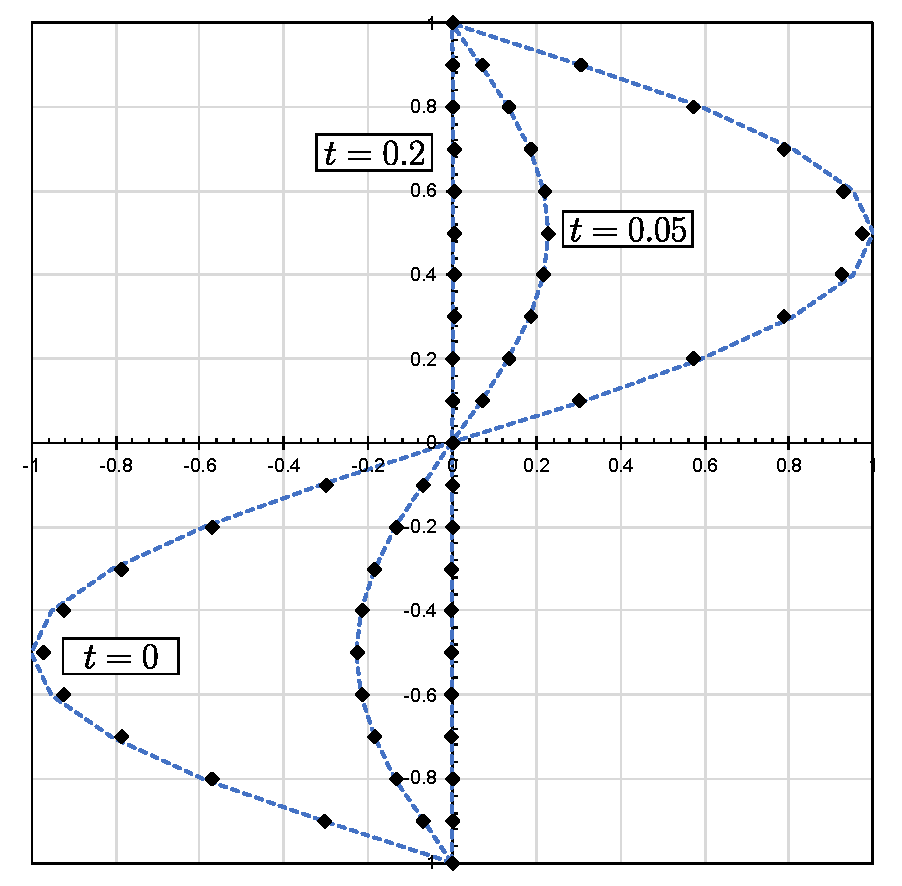
\includegraphics[width=\linewidth]{Figuras/taylor-green/LES-uz.pdf}
        \caption{$l3$ para LES.}
    \end{subfigure}
    \begin{subfigure}{0.42\textwidth}
        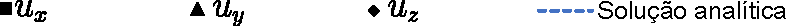
\includegraphics[width=\linewidth]{Figuras/taylor-green/legenda.pdf}
    \end{subfigure}
    \\Fonte: Autoria Própria (\the\year).
    \label{fig:TGV-results}
\end{figure}

Para comparação com a solução analítica, tomou-se a medida do erro em $L^2$, expresso por \cite{dumon2011proper}:

\begin{equation}
    \norm{\BB{e}}=\norm{\BB{u}-\BB{u}_a}_{L^\infty(L^2(\Omega))}=\max_{0<t\leq T}{\left[\int_\Omega{\norm{\BB{u}-\BB{u}_a}^2d\Omega}\right]}\text{,}
\end{equation}

\noindent o qual é representado ao longo do tempo de acordo com a Figura \ref{fig:TGV-L2}:

\begin{figure}[h!]
    \centering
    \caption{Medidas de $L^2$ ao longo do tempo.}
    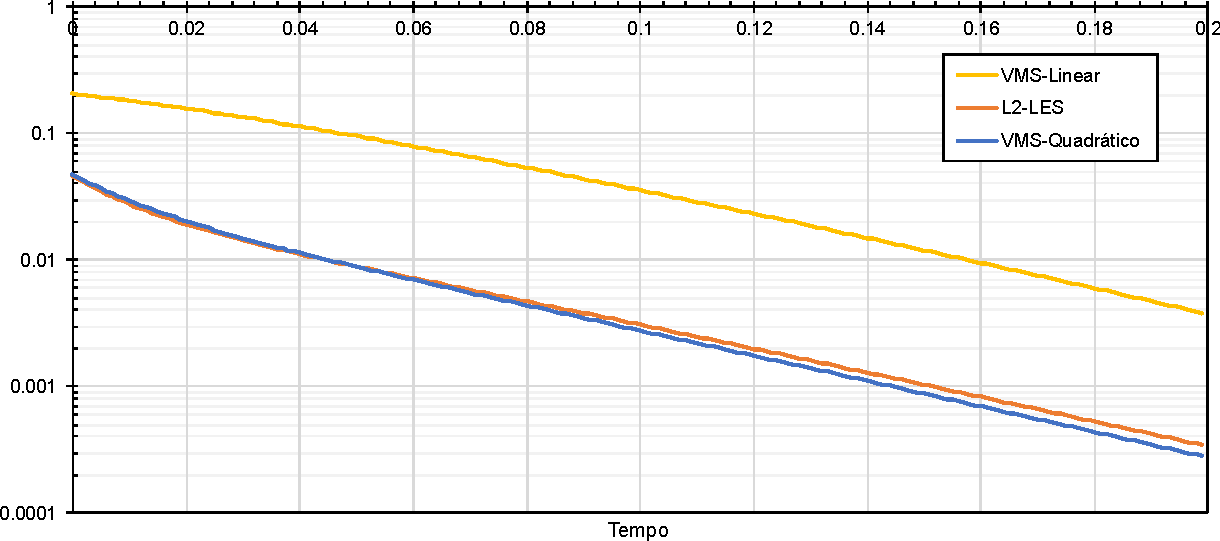
\includegraphics[width=\linewidth]{Figuras/taylor-green/L2.pdf}
    \\Fonte: Autoria Própria (\the\year).
    \label{fig:TGV-L2}
\end{figure}

Assim, observa-se que para o problema estudado, tanto as simulações VMS de aproximação quadrática quanto LES com elemento P2P1 apresentaram boa concordância com o resultado analítico, sendo que ambos apresentaram erros muito próximos entre si, enquanto o VMS de aproximação linear já apresentou um erro maior. Analisando o instante de tempo $t=0.1$ obteve-se um erro $L^2$ de $3,55\times 10^{-2}$, $2,77\times 10^{-3}$ e $3,07\times 10^{-3}$ para as simulações VMS linear, quadrático e LES, respectivamente. Ao verificar a ordem da medida do erro, observa-se que estes valores encontram-se próximos ao obtido por \citeonline{zapata2023parallel}. Realizando uma regressão exponencial do tipo \[\norm{\BB{e}}=a\cdot10^{mt}\] para $t\geq 0,1$, encontra-se $m=-9,80$, $m=-10,01$ e $m=-9,60$ para os respectivos modelos.

%==================================================================================================
\subsubsection{Escoamento sobre um cilindro}
%==================================================================================================

Para o seguinte problema considerou-se um cilindro circular de raio $R=0,5$ em um domínio retangular $\Omega=[0,112R]\times[0,100R]$, sendo o centro do cilindro posicionado sobre o ponto $(36,50)R$. As condições de contorno consideradas foram de entrada na face esquerda ($x_1=0$) do domínio ($\BB{u}=\{u_\infty,0\}^T$), condição de velocidade vertical nula nas faces inferior e superior ($u_2=0$ em $x_2=0$ e $x_2=100R$) e pressão nula no ponto $(112,100)R$. Como condição inicial aplicou-se uma velocidade $\BB{u}=\{u_\infty,0\}^T$ em todo o domínio. A densidade do fluido foi de $\rho=1$ com viscosidade $\nu=0,01$ e uma velocidade $u_\infty=1$, que, ao considerar o comprimento característico como o diâmetro do cilindro, obtém-se $\Rey=100$.

Para a simulação numérica, considerou-se a malha apresentada na Figura \ref{fig:cyl-mesh}, a qual possui 8106 elementos finitos, simulada em VMS de aproximação linear (12546 graus de liberdade), quadrática (49410 graus de liberdade) e LES com elemento P2P1 (37122 graus de liberdade). O intervalo de tempo foi de $t\in[0,200]$ com passos de $\Delta t=0,1$.

\begin{figure}[h!]
    \centering
    \caption{Malha utilizada para a simulação de escoamento sobre um cilindro.}
    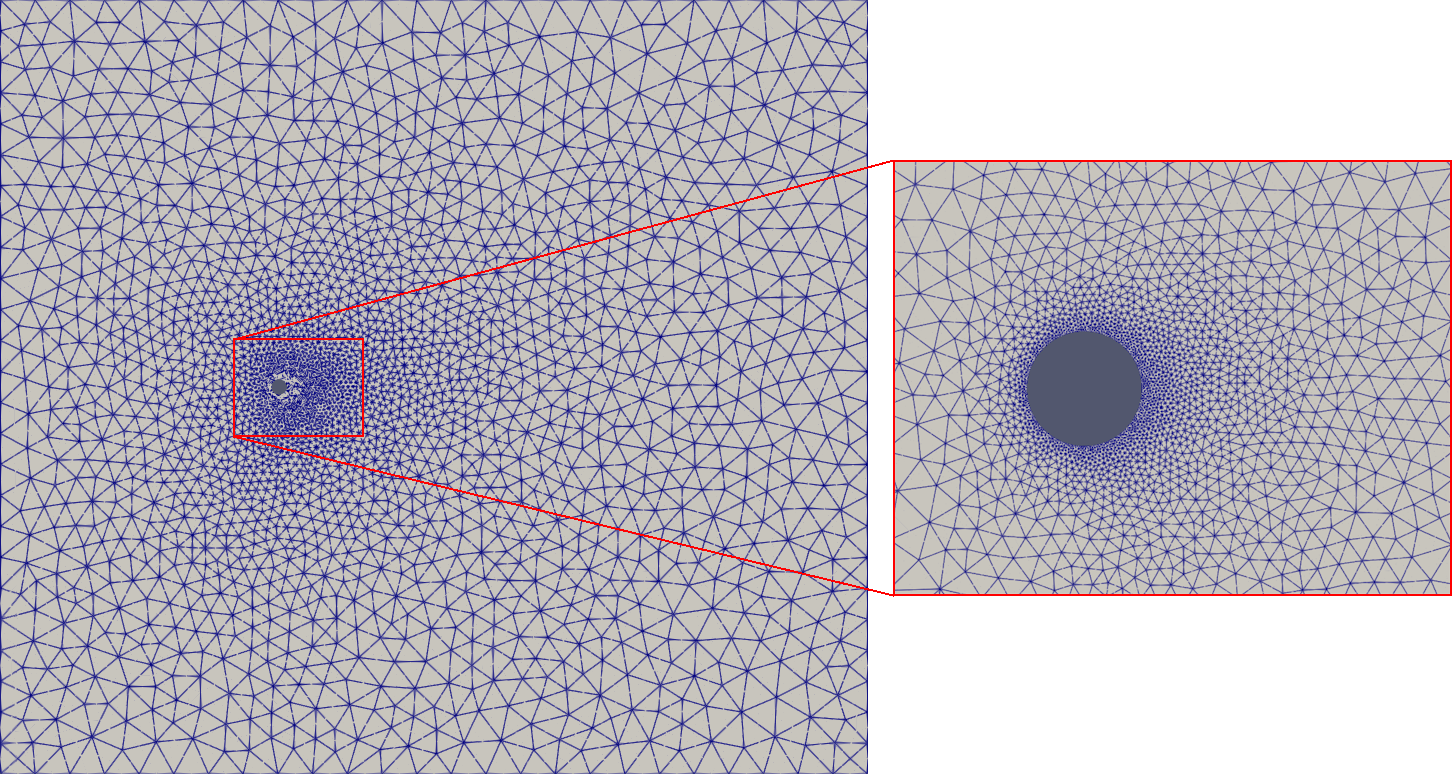
\includegraphics[width=\linewidth]{Figuras/cylinder/mesh.png}
    \\Fonte: Autoria Própria (\the\year).
    \label{fig:cyl-mesh}
\end{figure}

Para análise dos resultados determinou-se os coeficientes de arrasto (\textit{Drag} $C_D$) e de sustentação (\textit{lift} $C_L$), dados respectivamente por:

\begin{subequations}
    \begin{equation}
        C_D=\frac{2F_D}{\rho\norm{\BB{u}_\infty}^2L}\text{ e}
    \end{equation}
    \begin{equation}
        C_L=\frac{2F_L}{\rho\norm{\BB{u}_\infty}^2L}\text{,}
    \end{equation}
\end{subequations}

\noindent em que $F_D$ e $F_L$ são as forças de arrasto e de sustentação, calculados como:

\begin{subequations}
    \begin{equation}
        F_D=\int_{\Gamma_S}{\BB{\sigma}_{1j}n_jd\Gamma_S}\text{ e}
    \end{equation}
    \begin{equation}
        F_L=\int_{\Gamma_S}{\BB{\sigma}_{2j}n_jd\Gamma_S}\text{,}
    \end{equation}
\end{subequations}

\noindent sendo $\Gamma_S$ a fronteira do cilindro e $\BB{n}$ o vetor normal à $\Gamma_S$.

Outro parâmetro possível de se verificar é o número de Strouhal ($\Str$), que se trata de um número adimensional que busca relacionar a frequência de oscilação devido à formação de vórtices e a velocidade do fluido. Esse parâmetro pode ser determinado por:

\begin{equation}
    \Str=\frac{f_vL}{\norm{\BB{u}_\infty}}\text{,}
\end{equation}

\noindent sendo $f_v$ a frequência de desprendimento de vórtices.

A Figura \ref{fig:cyl-draglift} apresenta os coeficientes de arrasto e de sustentação obtidos na simulações e as Figuras \ref{fig:cyl-res1} e \ref{fig:cyl-res2} apresentam os campos de velocidades e de pressões atuantes no cilindro nos intantes $t=60$ e $t=120$.

\begin{figure}[h!]
    \centering
    \caption{Valores ao longo do tempo de:}
    \begin{subfigure}{\textwidth}
        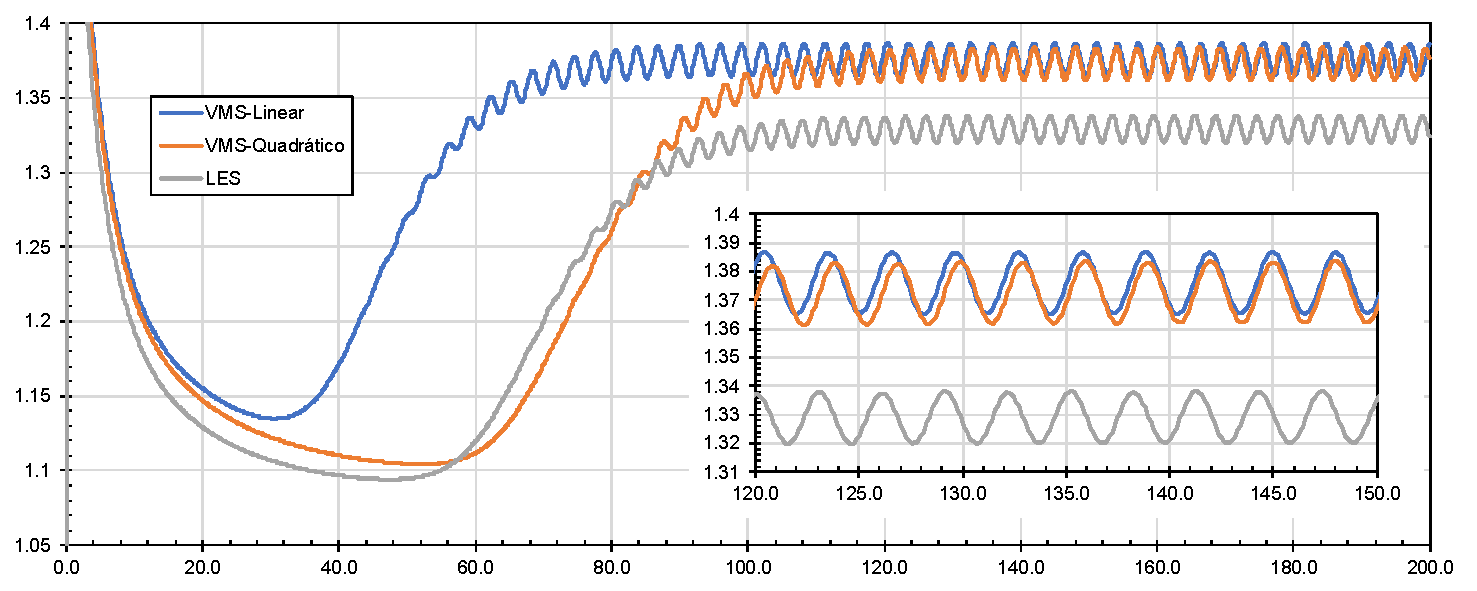
\includegraphics[width=\linewidth]{Figuras/cylinder/drag.pdf}
        \caption{coeficiente de arrasto.}
    \end{subfigure}
    \begin{subfigure}{\textwidth}
        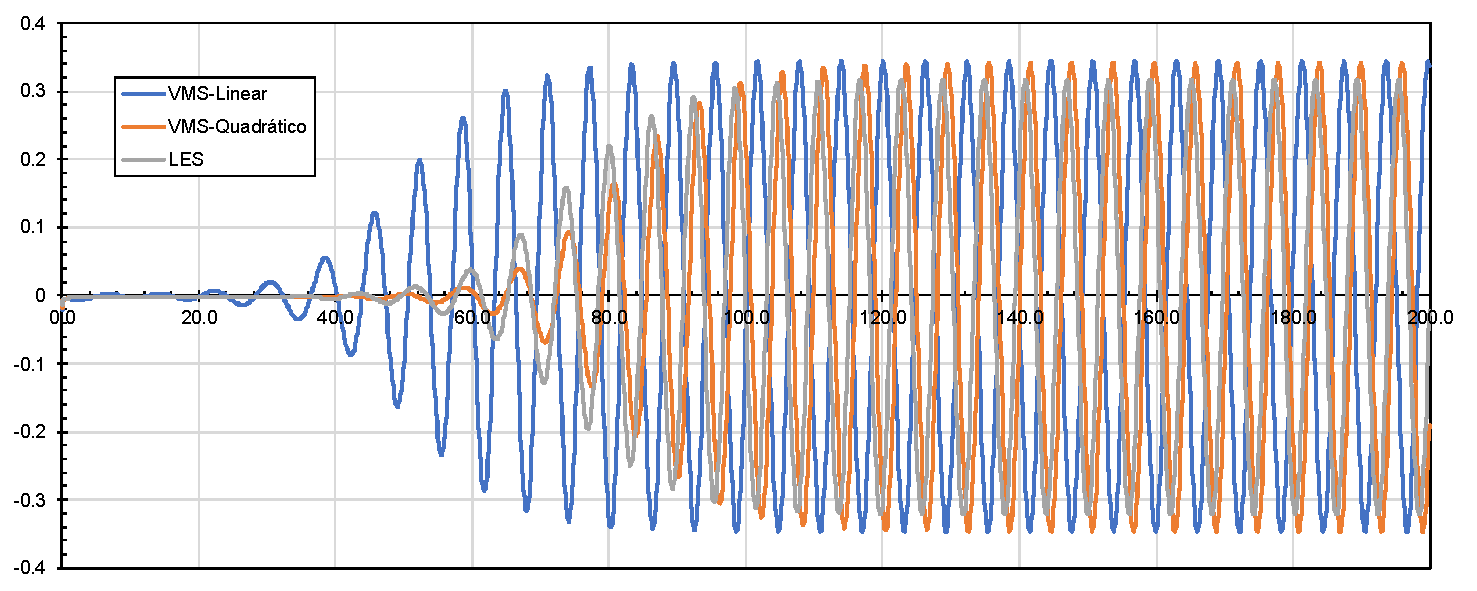
\includegraphics[width=\linewidth]{Figuras/cylinder/lift.pdf}
        \caption{coeficiente de sustentação.}
    \end{subfigure}
    \\Fonte: Autoria Própria (\the\year).
    \label{fig:cyl-draglift}
\end{figure}

\begin{figure}[h!]
    \centering
    \caption{Resultados no instante $t=60$.}
    \begin{subfigure}{\textwidth}
        \begin{subfigure}{\textwidth}\centering
            \begin{subfigure}{.42\textwidth}
                \caption*{Campo de velocidades.}
                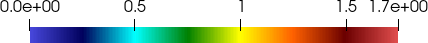
\includegraphics[width=\linewidth]{Figuras/cylinder/Legenda-vel.png}
            \end{subfigure}
            \begin{subfigure}{.42\textwidth}
                \caption*{Campo de pressões.}
                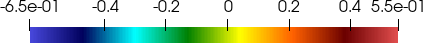
\includegraphics[width=\linewidth]{Figuras/cylinder/Legenda-pre.png}
            \end{subfigure}
        \end{subfigure}
    \end{subfigure}
    \begin{subfigure}{\textwidth}\centering
        \begin{subfigure}{.42\textwidth}
            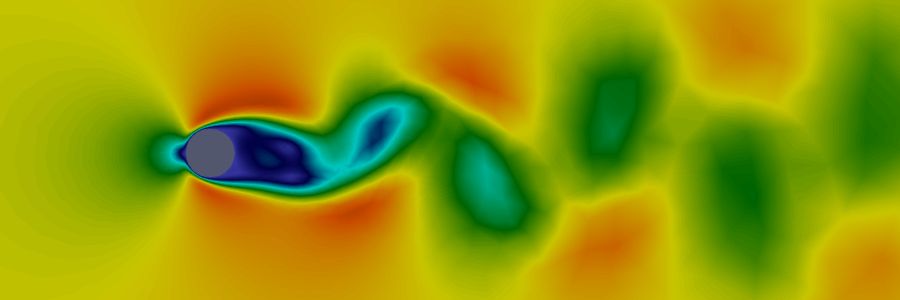
\includegraphics[width=\linewidth]{Figuras/cylinder/VMS-Lin-vel.png}
        \end{subfigure}
        \begin{subfigure}{.42\textwidth}
            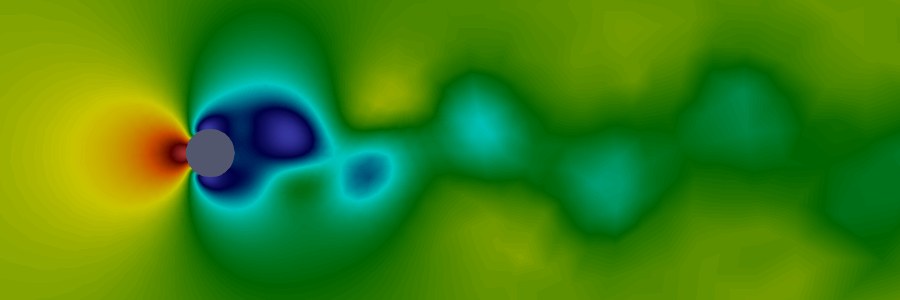
\includegraphics[width=\linewidth]{Figuras/cylinder/VMS-Lin-pre.png}
        \end{subfigure}
        \caption{VMS linear.}
    \end{subfigure}
    \begin{subfigure}{\textwidth}\centering
        \begin{subfigure}{.42\textwidth}
            \includegraphics[width=\linewidth]{Figuras/cylinder/VMS-Qua-vel.png}
        \end{subfigure}
        \begin{subfigure}{.42\textwidth}
            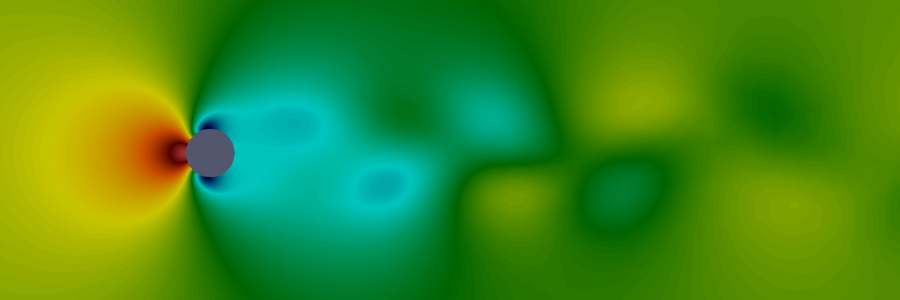
\includegraphics[width=\linewidth]{Figuras/cylinder/VMS-Qua-pre.png}
        \end{subfigure}
        \caption{VMS quadrático.}
    \end{subfigure}
    \begin{subfigure}{\textwidth}\centering
        \begin{subfigure}{.42\textwidth}
            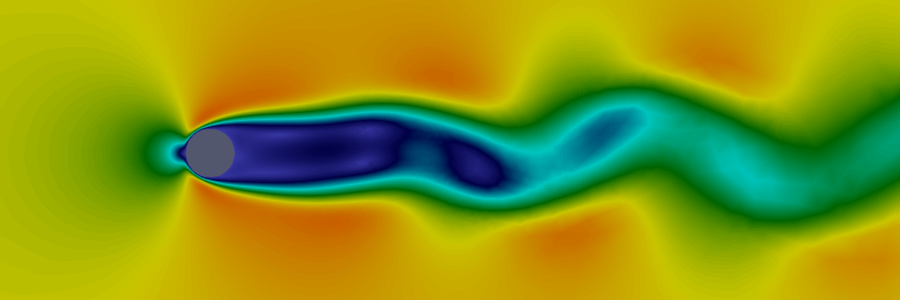
\includegraphics[width=\linewidth]{Figuras/cylinder/LES-vel.png}
        \end{subfigure}
        \begin{subfigure}{.42\textwidth}
            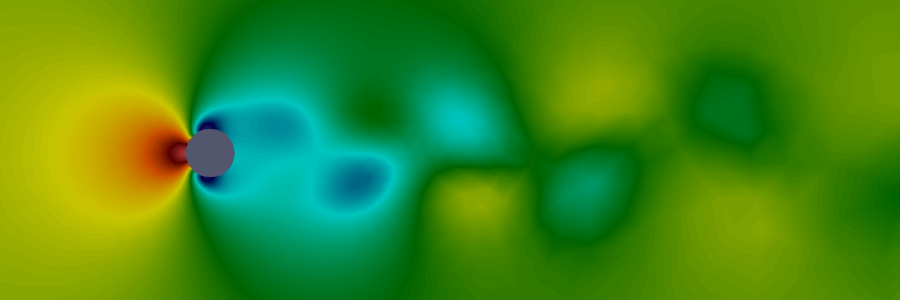
\includegraphics[width=\linewidth]{Figuras/cylinder/LES-pre.png}
        \end{subfigure}
        \caption{LES.}
    \end{subfigure}
    \\Fonte: Autoria Própria (\the\year).
    \label{fig:cyl-res1}
\end{figure}

\begin{figure}[h!]
    \centering
    \caption{Resultados no instante $t=120$.}
    \begin{subfigure}{\textwidth}\centering
        \begin{subfigure}{.42\textwidth}
            \caption*{Campo de velocidades.}
            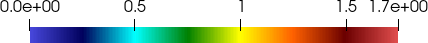
\includegraphics[width=\linewidth]{Figuras/cylinder/Legenda-vel.png}
        \end{subfigure}
        \begin{subfigure}{.42\textwidth}
            \caption*{Campo de pressões.}
            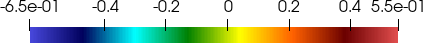
\includegraphics[width=\linewidth]{Figuras/cylinder/Legenda-pre.png}
        \end{subfigure}
    \end{subfigure}
    \begin{subfigure}{\textwidth}\centering
        \begin{subfigure}{.42\textwidth}
            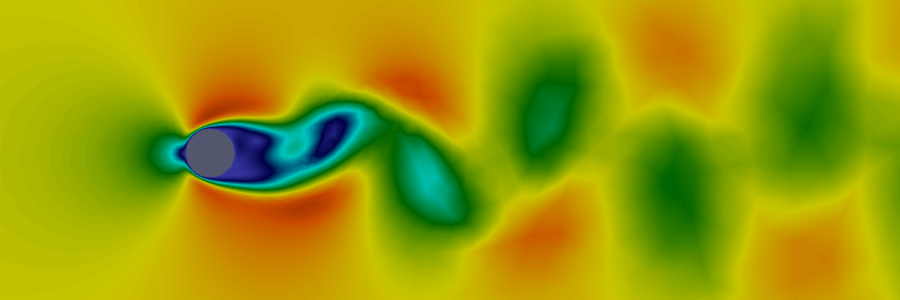
\includegraphics[width=\linewidth]{Figuras/cylinder/VMS-Lin2-vel.png}
        \end{subfigure}
        \begin{subfigure}{.42\textwidth}
            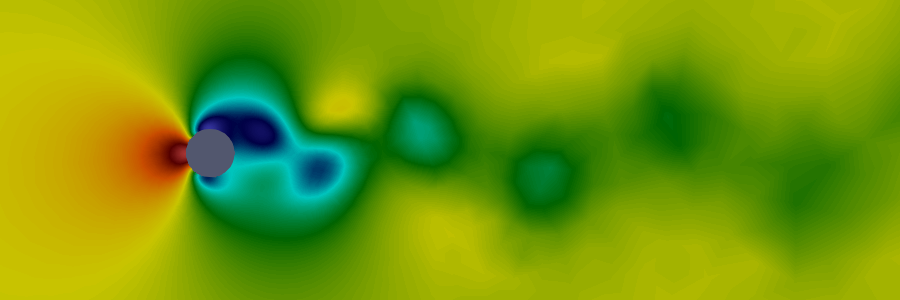
\includegraphics[width=\linewidth]{Figuras/cylinder/VMS-Lin2-pre.png}
        \end{subfigure}
        \caption{VMS linear.}
    \end{subfigure}
    \begin{subfigure}{\textwidth}\centering
        \begin{subfigure}{.42\textwidth}
            \includegraphics[width=\linewidth]{Figuras/cylinder/VMS-Qua2-vel.png}
        \end{subfigure}
        \begin{subfigure}{.42\textwidth}
            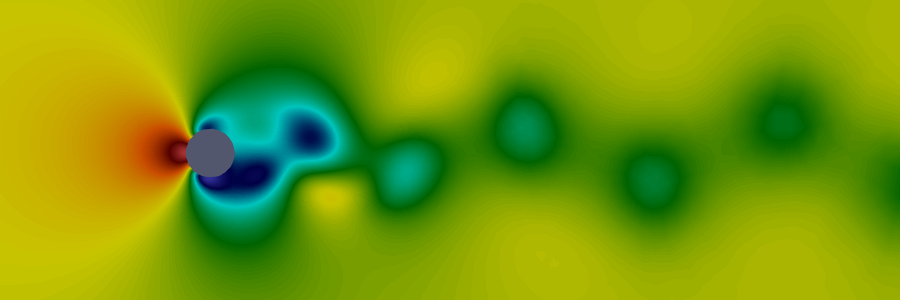
\includegraphics[width=\linewidth]{Figuras/cylinder/VMS-Qua2-pre.png}
        \end{subfigure}
        \caption{VMS quadrático.}
    \end{subfigure}
    \begin{subfigure}{\textwidth}\centering
        \begin{subfigure}{.42\textwidth}
            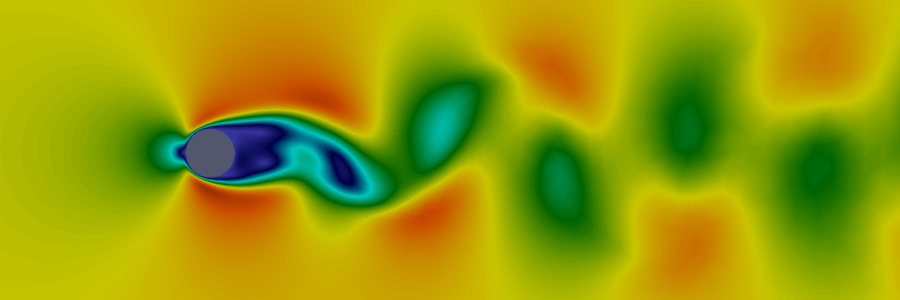
\includegraphics[width=\linewidth]{Figuras/cylinder/LES2-vel.png}
        \end{subfigure}
        \begin{subfigure}{.42\textwidth}
            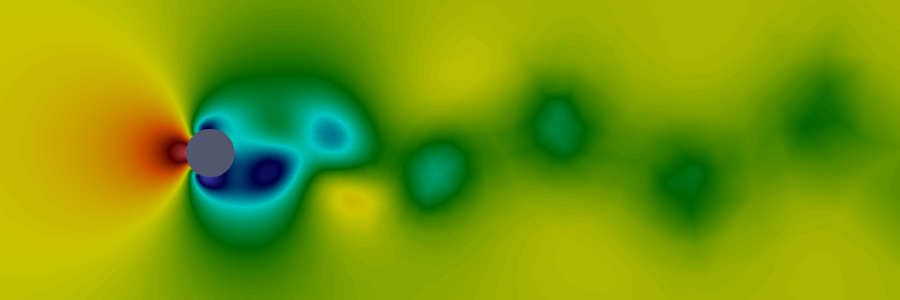
\includegraphics[width=\linewidth]{Figuras/cylinder/LES2-pre.png}
        \end{subfigure}
        \caption{LES.}
    \end{subfigure}
    \\Fonte: Autoria Própria (\the\year).
    \label{fig:cyl-res2}
\end{figure}

Os valores da média e da amplitude dos coeficientes de arrasto e de sustentação após o instante $t=120$, assim como o número de Strouhal são apresentados na Tabela \ref{tab:cyl-res}.

\begin{table}[h!]
    \centering
    \newcommand{\MR}{\multirow}
    \newcommand{\MC}{\multicolumn}
    \caption{Valores das propriedades dos coeficientes de arrasto e de sustentação para os modelos analisados.}
    \begin{tabular}{lcccccc}
        \hline
        \MC{1}{c}{}                   & \MC{2}{c}{VMS-Lin} & \MC{2}{c}{VMS-Qua} & \MC{2}{c}{LES}                                           \\ \cline{2-7}
        \MC{1}{c}{\MR{-2}{*}{Param.}} & Arrasto            & Sustentação        & Arrasto            & Sustentação & Arrasto & Sustentação \\ \hline
        Amplitude                     & 0,01083            & 0,34519            & 0,01130            & 0,34377     & 0,00930 & 0,31968     \\
        Média                         & 1,37590            & -0,00009           & 1,37273            & -0,00760    & 1,32901 & -0,00464    \\
        Strouhal                      & \MC{2}{c}{0,16393} & \MC{2}{c}{0,16667} & \MC{2}{c}{0,16393}                                       \\ \hline
    \end{tabular}
    \\Fonte: Autoria Própria (\the\year).
    \label{tab:cyl-res}
\end{table}

Comparando-se os números de Strouhal calculados com aqueles obtidos por \citeonline{tezduyar1992incompressible}, os quais verificaram $\Str$ entre 0,166 e 0,170, \citeonline{najafi2012meshless}, com valor de 0,182, e \citeonline{codina2006numerical}, com velores entre 0,177 e 0,184. As variações observadas entre os resultados dos diferentes autores podem ser devidas às diferenças nas dimensões dos domínios utilizados, assim como as diferentes condições de contorno aplicadas por cada um. No entanto ainda observa-se que em todos os casos os valores calculados nas simulações ainda são bem próximos. Vale observar ainda que a simulação VMS linear apresentou um amortecimento menor em relação ao início das oscilações, porém converge para valores muito próximos ao quadrático ao longo do tempo. Já a simulação LES inicia sua oscilação próxima ao VMS quadrático, entretanto com uma média de oscilação menor que a do VMS, em especial ao se observar o coeficiente de arrasto. Tal efeito pode ser devido ao relatado por \citeonline{germano1991dynamic,hughes2000large}, que apontam a ocorrência de um amortecimento excessivo provocado pelo tensor SGS de Smagorinsky.